% Plantilla creada por Eduardo Mosqueira Rey
%
% Libro online bastante completo para consulta de Latex: http://en.wikibooks.org/wiki/LaTeX/
% Versión en castellano: http://es.wikibooks.org/wiki/Manual_de_LaTeX
\documentclass[12pt, a4paper, titlepage]{article}

\usepackage[spanish]{babel} % Soporte multilenguaje para LaTeX.

\usepackage[a4paper, top=2.5cm, bottom=2.5cm, left=2.5cm, right=2.5cm]{geometry} % Interfaz flexible para definir las dimensiones del documento

\usepackage[utf8]{inputenc} % Aceptar diferentes tipos de codificación de caracteres de entrada (en este caso usamos la codificación Unicode UTF-8)

\usepackage{graphicx} % Soporte aumentado para gráficos 
\usepackage{hyperref}
\usepackage{captdef}
\begin{document}

%%%%%%%%%%%%%%%%%%%%%%%%%%%%%%%%%%%%%%%%%%%%%%%%%%%%%%%%%%%%%%%%%%%%%%%%%%%%%%%%
% PORTADA
%%%%%%%%%%%%%%%%%%%%%%%%%%%%%%%%%%%%%%%%%%%%%%%%%%%%%%%%%%%%%%%%%%%%%%%%%%%%%%%%

\begin{titlepage}


\includegraphics[width=15cm]{Imagenes/Simbolo_logo_UDC.png}

% Lista de tamaños: \Huge, \huge, \LARGE, \Large, \large, \small, \footnotesize, \tiny
\vspace{3cm}

\begin{center}

\includegraphics[scale=0.3]{Imagenes/1a_Practica_ER_14-15.png}
\end{center}


\begin{flushright}
	
	\LARGE{\textbf{ JoinMe!}}
	
	\LARGE{\textbf{StoryBoards y Prototipos del interfaz del Usuario
	}}
	
	\large{\textbf{Version 1.0}}
	
\end{flushright}

\vspace{1cm}
\begin{center}
José Antonio López Sebio\\
Pablo Paz Varela\\
Grupo ER-12-03\\
\end{center}

\vspace{2cm}

\begin{center}
	\large{\textbf{Histórico}}
	
    \begin{tabular}{ | p{4cm} | p{2cm} | p{6cm} | p{3cm} |}
    \hline
    \textbf{Fecha} & \textbf{Version} & \textbf{Descripción} & \textbf{Autor} \\ \hline
      14/05/2014 & 1.0 & Primera Revisión & ER-12-03\\ \hline
      &  &  & \\ \hline
     &  & &\\ \hline
    \end{tabular}
\end{center}


\end{titlepage}
\clearpage

%%%%%%%%%%%%%%%%%%%%%%%%%%%%%%%%%%%%%%%%%%%%%%%%%%%%%%%%%%%%%%%%%%%%%%%%%%%%%%%%
% INDICE
%%%%%%%%%%%%%%%%%%%%%%%%%%%%%%%%%%%%%%%%%%%%%%%%%%%%%%%%%%%%%%%%%%%%%%%%%%%%%%%%

\tableofcontents
\clearpage

%%%%%%%%%%%%%%%%%%%%%%%%%%%%%%%%%%%%%%%%%%%%%%%%%%%%%%%%%%%%%%%%%%%%%%%%%%%%%%%%
\section{Introducción}
%%%%%%%%%%%%%%%%%%%%%%%%%%%%%%%%%%%%%%%%%%%%%%%%%%%%%%%%%%%%%%%%%%%%%%%%%%%%%%%%

%**********************************************************
\subsection{Propósito}
%**********************************************************
Este documento tiene por propósito mostrar los \textit{Storyboards} de los casos de uso implementados de la red social \textbf{JoinMe!} además de los \textit{Mockups} del diseño de la interfaz.



%**********************************************************
\subsection{Definiciones, Acrónimos y Abreviaturas}
%**********************************************************

Consultar Glosario de términos.

%**********************************************************
\subsection{Referencias}
%**********************************************************

\begin{itemize}

    \item JoinMe! - Glosario
    \item JoinMe! - Modelo de casos de uso
    \item JoinMe! - Especificación suplementaria
    \item JoinMe! - Modelo del dominio
\end{itemize}

\newpage
\section{Storyboards}

\subsection{Registrarse en la red social}

\begin{figure}[h]
	\begin{center}
		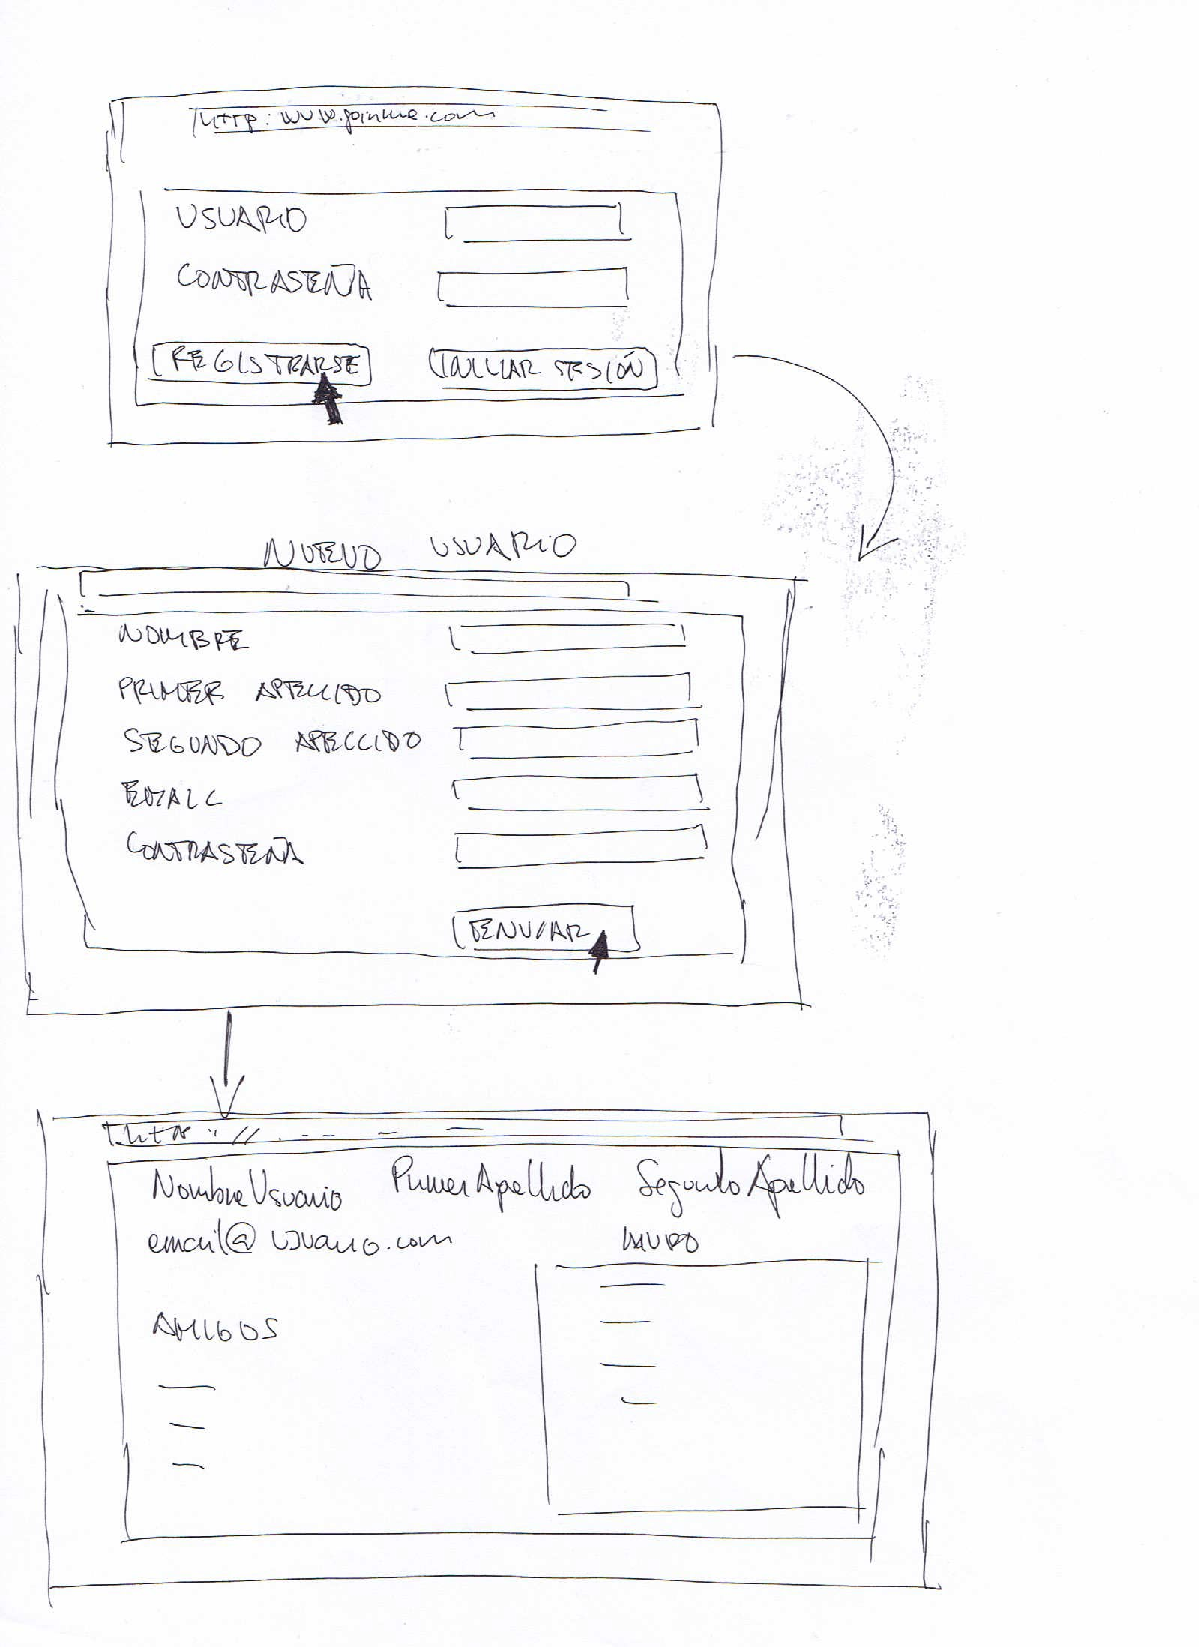
\includegraphics[scale=0.6]{Imagenes/registrarse}
		\caption{Storyboard Registrarse en la red social.}
	\end{center}
\end{figure}

\clearpage

\subsection{Enviar petición de amistad}


	\begin{center}
		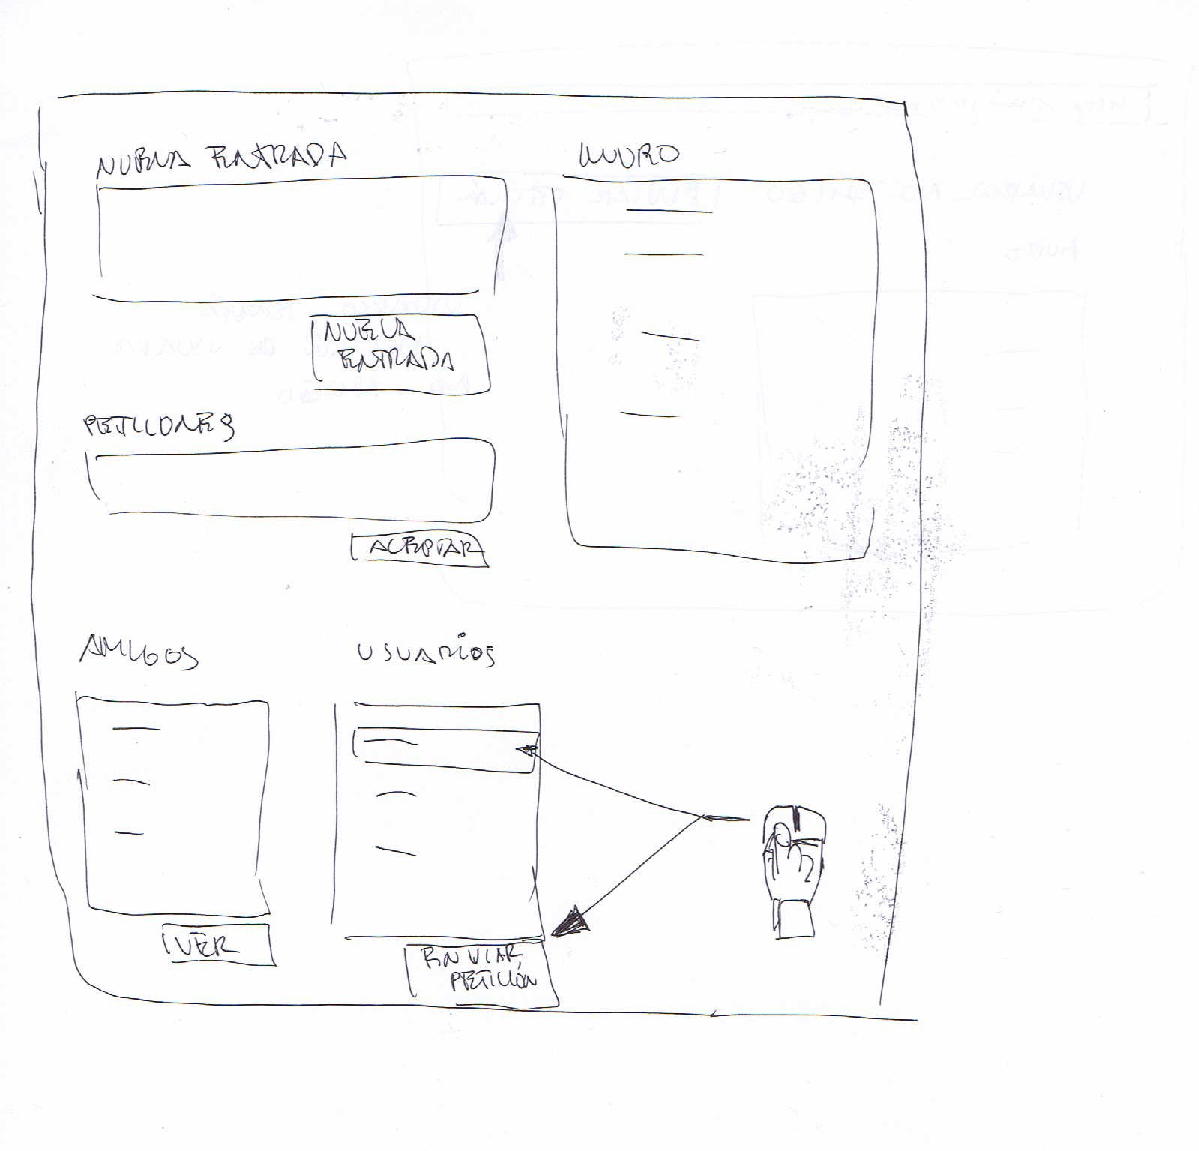
\includegraphics[scale=0.6]{Imagenes/enviar_peticion_no_amigo}
		\figcaption{Storyboard enviar petición a usuario no amigo 1.}
	\end{center}



	\begin{center}
		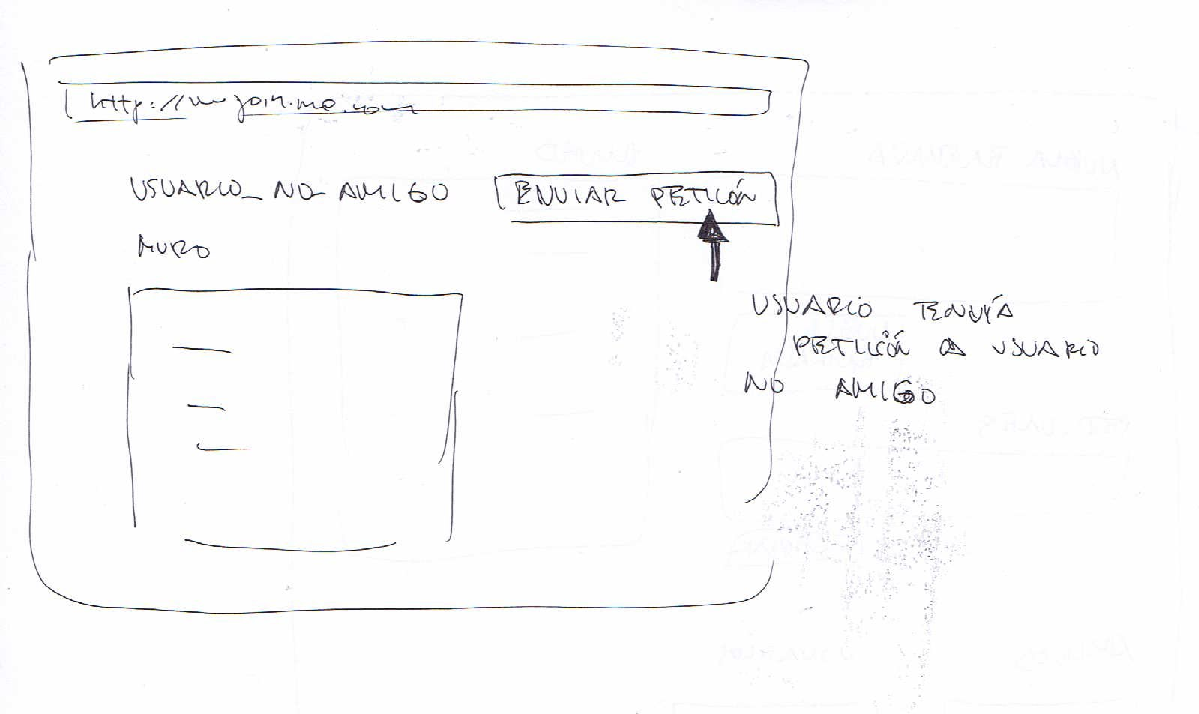
\includegraphics[scale=0.6]{Imagenes/enviar_peticion_no_amigo_2}
		\figcaption{Storyboard enviar petición a usuario no amigo 1.}
	\end{center}

\subsection{Ver muro amigo y lista de amigos}


	\begin{center}
		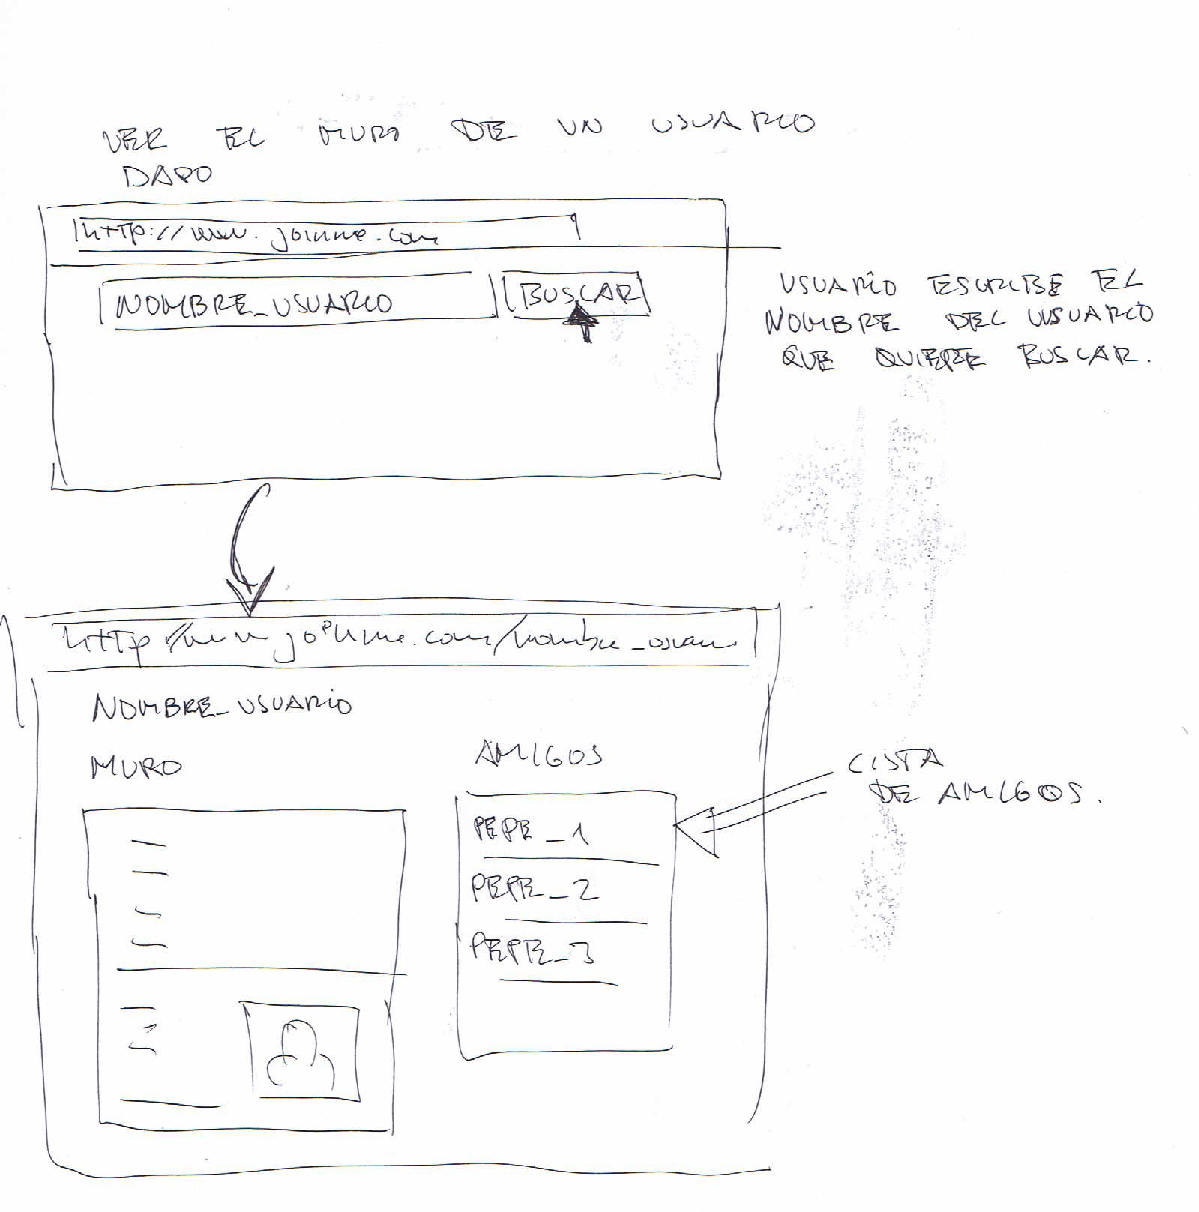
\includegraphics[scale=0.5]{Imagenes/ver_muro_amigo}
		\figcaption{Storyboard ver muro de un amigo.}
	\end{center}


\subsection{Publicar nueva entrada}

	\begin{center}
		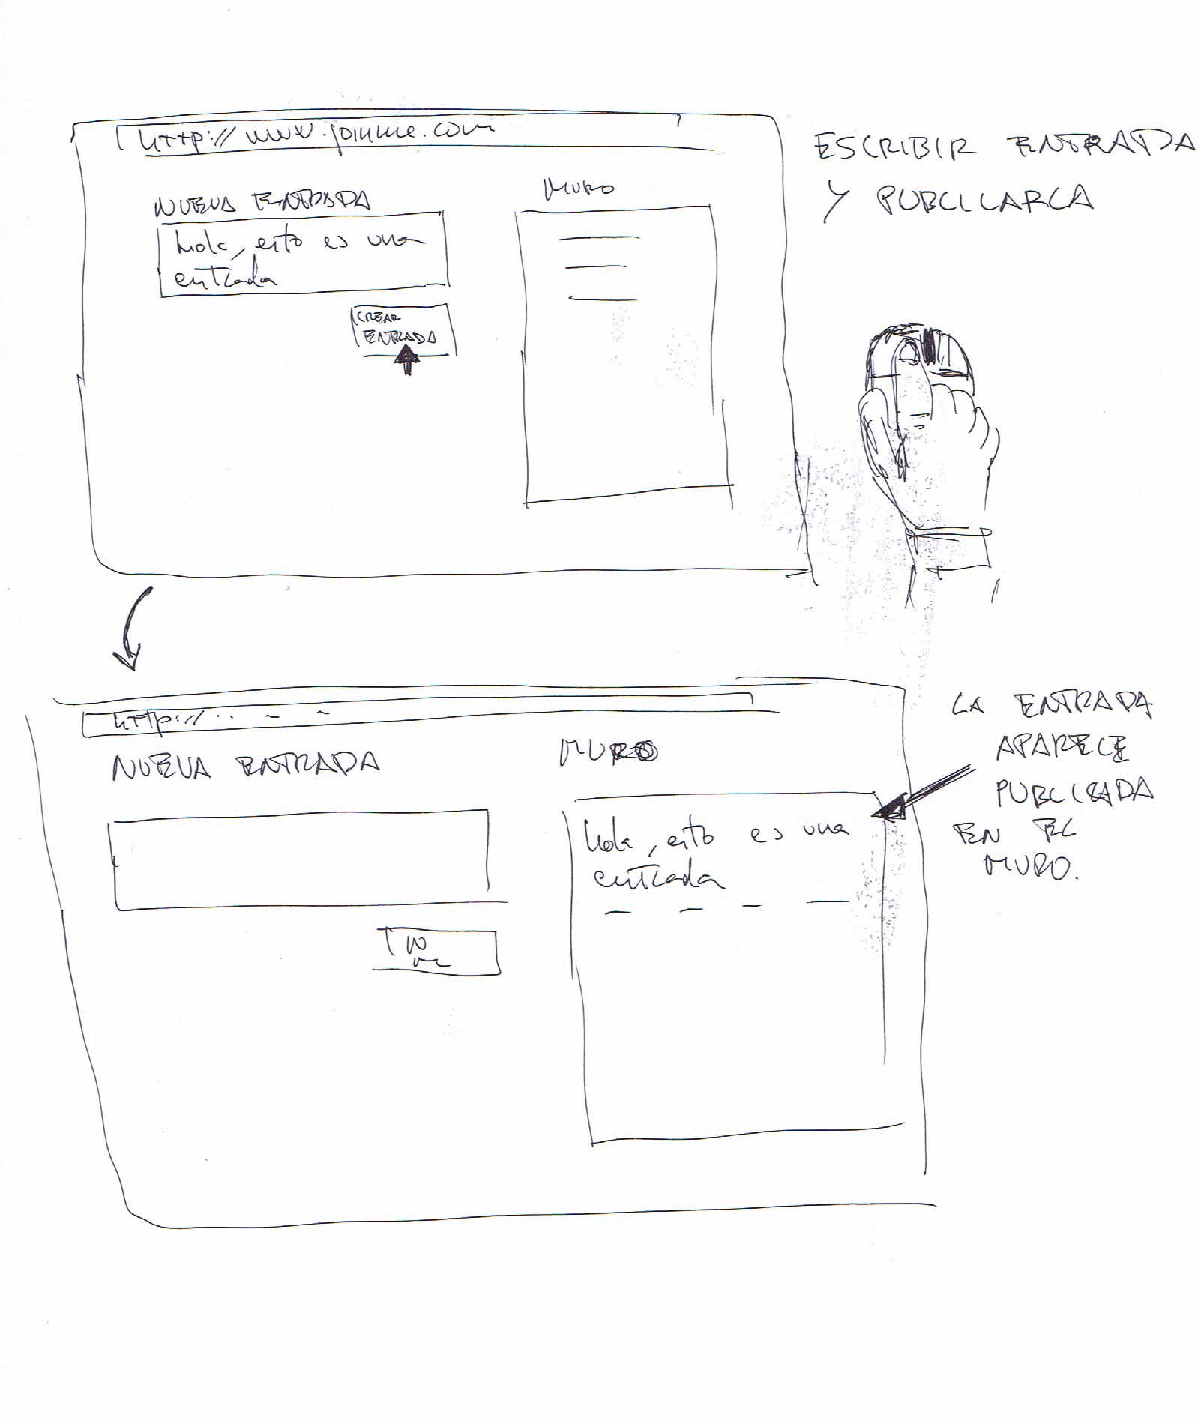
\includegraphics[scale=0.5]{Imagenes/nueva_entrada}
		\figcaption{Storyboard Registrarse en la red social.}
	\end{center}

\clearpage
\section{Mockups}

\subsection{Inicio sesión}

\begin{center}
	
	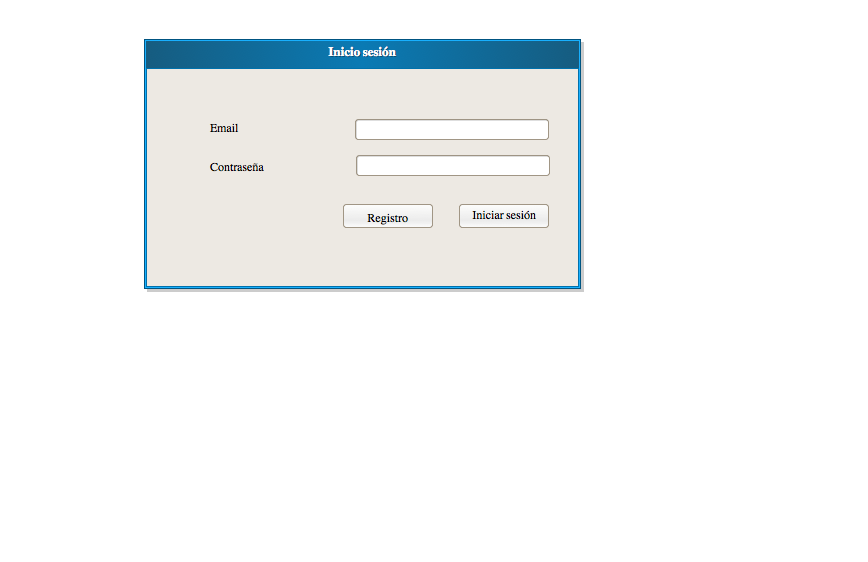
\includegraphics[scale=0.7]{Imagenes/Ventana_inicio_sesion.png}
	\figcaption{Mockup Ventana inicio sesión}
	
\end{center}

\subsection{Nuevo usuario}

\begin{center}
	
	\includegraphics[scale=0.7]{Imagenes/registro.png}
	\figcaption{Mockup Ventana nuevo usuario}
	
\end{center}

\subsection{Muro}

\begin{center}
	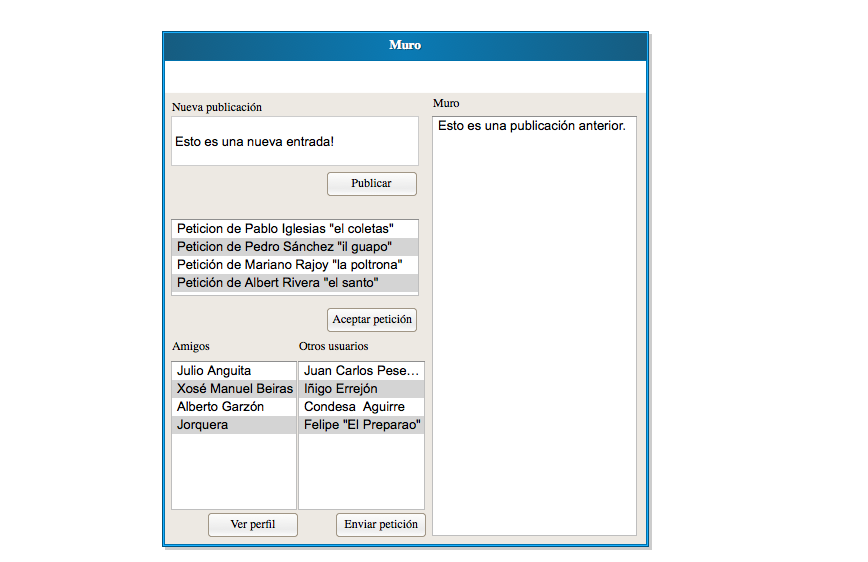
\includegraphics[scale=0.7]{Imagenes/muro}
	\figcaption{Mockup ventana principal del muro}
\end{center}

\subsection{Perfil usuario amigo}

\begin{center}
	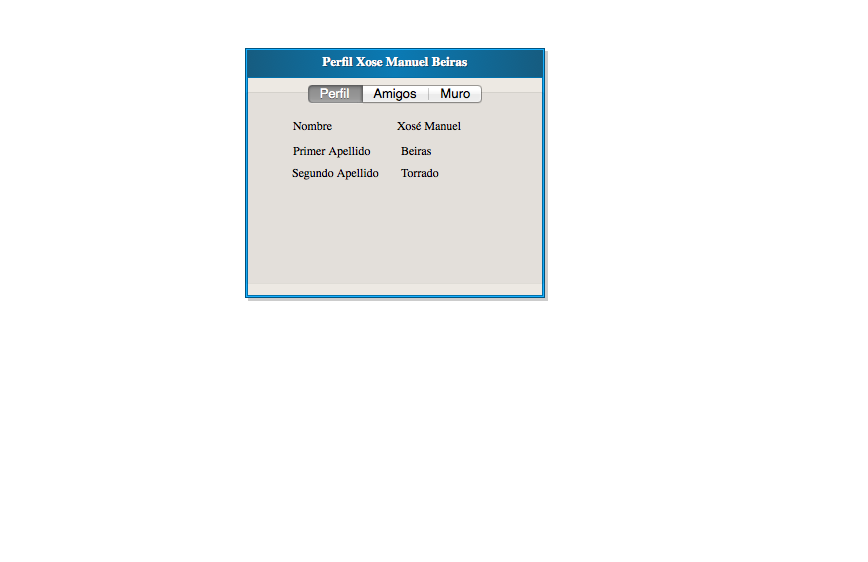
\includegraphics[scale=0.7]{Imagenes/perfil_amigo}
	\figcaption{Mockup ventana principal del  perfil de un amigo}
\end{center}

\begin{center}
	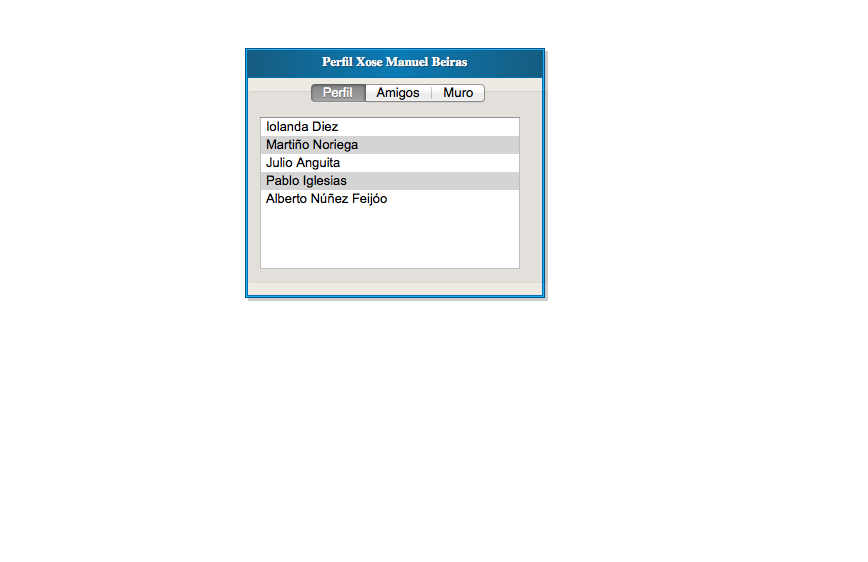
\includegraphics[scale=0.7]{Imagenes/perfil_amigo_amigos}
	\figcaption{Mockup ventana amigos del perfil de un amigo}
\end{center}

\begin{center}
	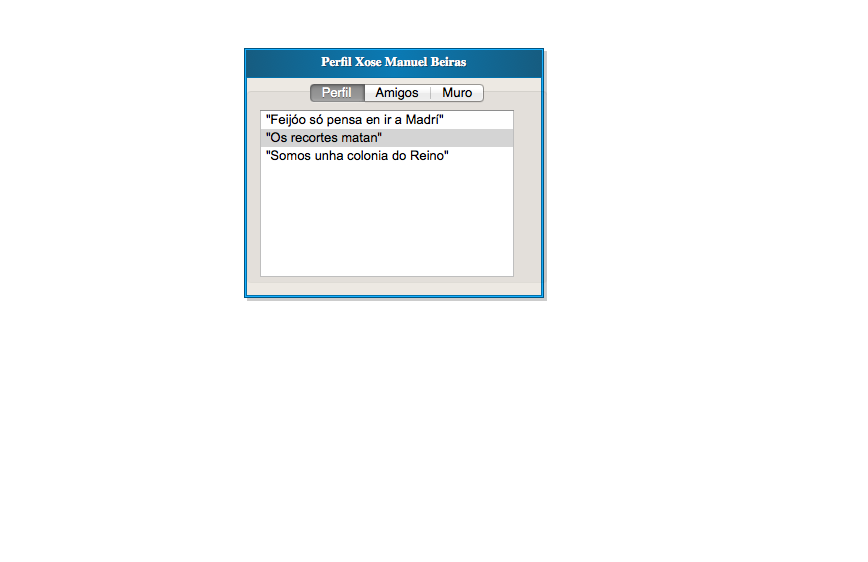
\includegraphics[scale=0.7]{Imagenes/perfil_amigo_muro}
	\figcaption{Mockup ventana muro del  perfil de un amigo}
\end{center}

\end{document}